\documentclass{beamer}

%\usepackage[latin2]{inputenc}
%\usepackage[T1]{fontenc}
\usepackage{amsmath,amssymb} % AMS matematikai és fontcsomag
\usepackage{amsthm}          % tételszerű környezetek
\usepackage{graphicx}        % képek beillesztéséhez
\usepackage{geometry}        % méretek állítása
\usepackage{subcaption} 	 % subfigure
\usetheme{Antibes}
\useoutertheme{miniframes} % Alternatively: miniframes, infolines, split
\useinnertheme{circles}
\usecolortheme{beaver}

\newtheorem{thm}{Theorem}
\newtheorem{defi}[thm]{Definition}
\newtheorem{lem}[thm]{Lemma}
\newtheorem{cor}[thm]{Corollary}
\newtheorem{prop}[thm]{Proposition}
\newtheorem{rem}[thm]{Remark}

\def\IR{\mathbb{R}}
\def\IT{\mathbb{T}}
\def\IN{\mathbb{N}}
\def\IZ{\mathbb{Z}}
\def\SS{\mathbb{S}}


\title{Analyzing the evolution of the European Parliament Social Network}

\date{2023-11-10}

\author{Á. Bernát, M. Marits}

\usepackage{graphicx}

%\setbeamertemplate{background}{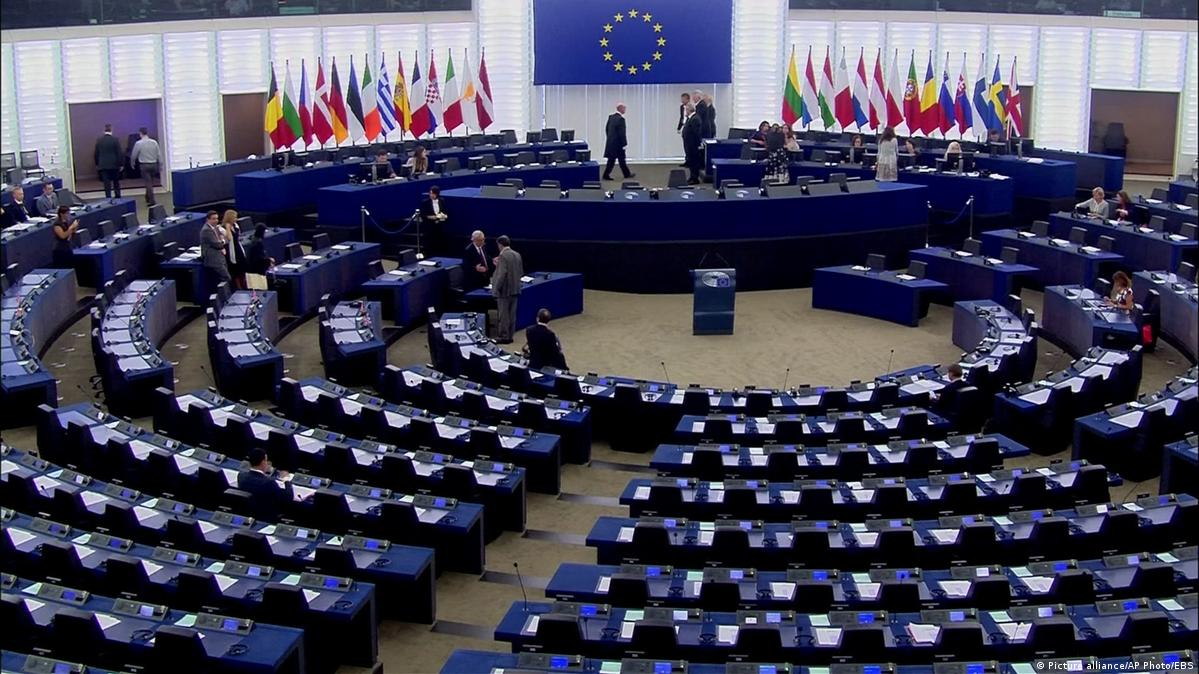
\includegraphics[width=\paperwidth,height=\paperheight,keepaspectratio]{img/euparl.jpg}}

\begin{document}
\begin{frame}[plain]
    \maketitle
\end{frame}

\begin{frame}{Introduction}
	
	\begin{figure}
		The European Parliament
	
		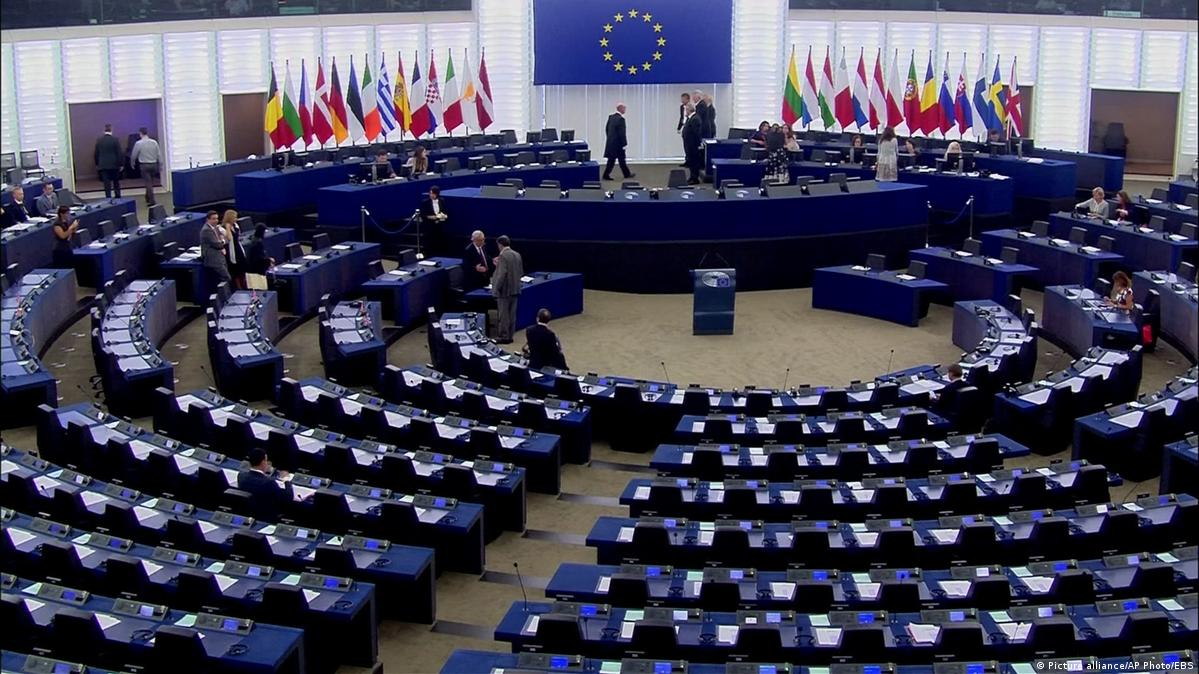
\includegraphics[width=0.5\textwidth]{img/euparl.jpg}
	\end{figure}

	We are analyzing a dataset of European Parliament members.
	
	\vspace{2mm}
	
	Our dataset is a list of ammendments.

	
\end{frame}

\begin{frame}
\frametitle{Our analysis}

\begin{columns}

\column{5cm}

We acquired data regarding amendments, for each amendment we know which MEP proposed the amendment, what kind of document it is, etc..
\bigskip

\pause Basically, we got a bipartite graph with node groups:
\begin{itemize}
	\item MEPs
	\item Documents
\end{itemize}
\bigskip

\pause Edges $\iff$ MEP made amendment to document

\pause \column{5cm}
\begin{center}
\small{A bipartite graph:}
\bigskip
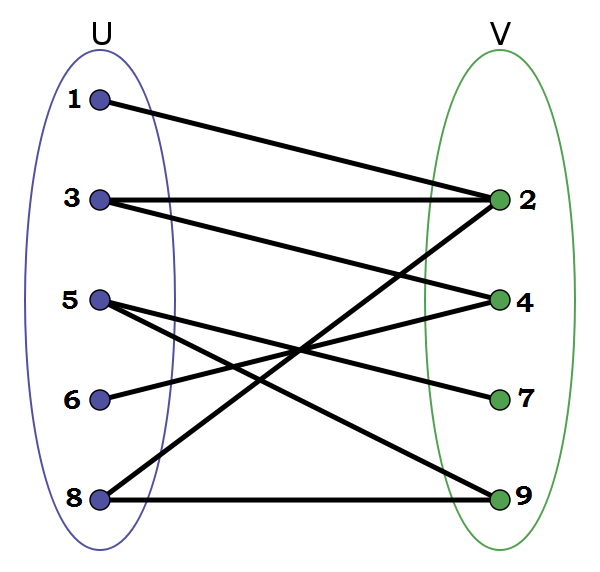
\includegraphics[height=3.2cm]{img/BipartiteGraph.png}
\end{center} 

\end{columns}
\end{frame}



\begin{frame}{Projection}

We then created a projection of this bipartite graph:

\begin{itemize}
	\pause \item Nodes: the nodes of MEPs
	\pause \item Edges: 2 MEPs are connected if they amended the same document	
\end{itemize}


%\pause We have also considered and implemented weighted projection. We used the so called: "Collaboration weighted projection"(where we reward secluded document matching and punish popular document matching)
%EZ nem tom kell e ? 

\end{frame}


\begin{frame}{Committees}

	What is a committee in the European Parliament?
	
	\pause They are groups of MEPs that work together on specific topics
	
	\pause Commitee members work together on a specific set of law changes
	
	\pause MEPs can join and leave committees at any time \pause (this makes this analysis non-trivial)
	
	\vspace{2mm}
	
	\pause Analysis of the EP has to take into account the committees, as they are important units for how work in the EP is distributed
	
\end{frame}

\begin{frame}{Important committees}
	
	The following are the largest and most influential committees in the EP: \pause \begin{itemize}
		\item Committee on Industry, Research and Energy (ITRE)
		\item Committee on the Environment, Public Health and Food Safety (ENVI)
		\item Committee on Foreign Affairs (AFET)
	\end{itemize}

	\pause We will try to analyze changes in the operations of these committees as well
	
\end{frame}

\begin{frame}{Motivation}

Understanding the network of MEPs might give us a better understanding of the following:

\bigskip

\begin{itemize}
	\pause \item How smaller networks inbetween MEPs look like, their size and their quantity.
	
	\pause \item \textbf{How events and occurrences shape the form and topology of the network.}
		
	\pause \item \textbf{How different groups behave within the network over time}

\end{itemize}

\pause All of these are helpful in understanding the processes regarding proposals and how they evolve into enacted laws.

\end{frame}

\begin{frame}{Analysis topic}
	
	We want to analyze the changes in the social network of the EP over time.
	
	\vspace{2mm}
	
	\pause For this, we picked two important properties of the network to investigate\begin{itemize}
		\pause \item Centrality of groups/MEPs
		
		\pause \item Cohesion of the network
	\end{itemize}
	
\end{frame}

\begin{frame}{Analyzing centrality in the network}
	
	Group centralities (similar to node centralities):
\begin{itemize}
	\pause \item Degree centrality 
	\[ 
		G = (V,E)\text{, } S \subset V \text{,  }\text{degree(S)} = \frac{|v \in V-S, \exists u \in S: uv \in E|}{|V-S|}	
	\]
	
	\pause \item Closeness centrality 
	\[
		S \subset V \text{,  }\text{closeness(S)} = \frac{|V-S|}{\sum_{u \in |V-S|}d_{S,u} }
	\]
		
	\pause \item Betweenness centrality

\end{itemize}
\end{frame}

\begin{frame}{Analyzing the cohesion of the network}
	
	Cohesion: a measure of how well-connected a network is
	
	\vspace{2mm}
	
	\pause Our measure of cohesion is that we find the proportion of edges that are present -- i.e. the proportion of MEP-pairs that worked together
	
	\pause \[
		\text{cohesion} = \frac{\#\text{edges}}{\binom{n}{2}}
	\]
	
\end{frame}


\begin{frame}{Subgraphs}
	We will measure the cohesion and centralities of certain subgraphs of the MEP social network.
	Which subset/subgraph did we consider ? 
	\begin{itemize}
	\pause \item Time intervals: Quarterly, Half-yearly (fixed early)
	\pause \item For each committee a different graph
	\pause \item Biggest component vs the whole graph
	\end{itemize}
\end{frame}


\begin{frame}{Assumptions}

Our initial assumptions are the following:
\bigskip
\begin{itemize}
	\pause \item The more a party is willing to cooperate with outside MEPs the more its centralities will be.

	\pause \item If one party has an interest in a particular topic, pushing its agenda will make it more central and cohesive
	
	\pause \item If a topic deeply divides the European Parliament then one would expect the centrality indexes of groups to dwindle 
\end{itemize}
\end{frame}

\begin{frame}{Our results: Centrality}
	
	Considering the \textbf{closeness} centralities of parties in the \textbf{quarterly} and \textbf{committee division}:
	\vspace{4mm}
	\pause
	
\begin{columns}
	\begin{column}{0.5\textwidth}
	Closeness of EPP party in ENVI:
	\\
	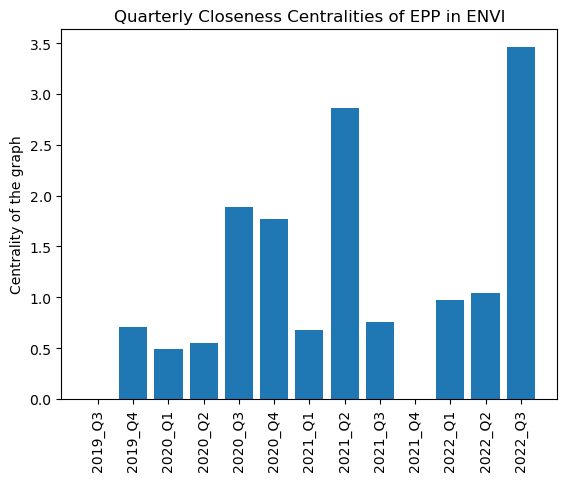
\includegraphics[width=\textwidth]{img/EPP_ENVI_Q_closeness.png}
	\end{column}
	
	\pause 
	\begin{column}{0.5\textwidth}
	Closeness of S\&D in ENVI:
	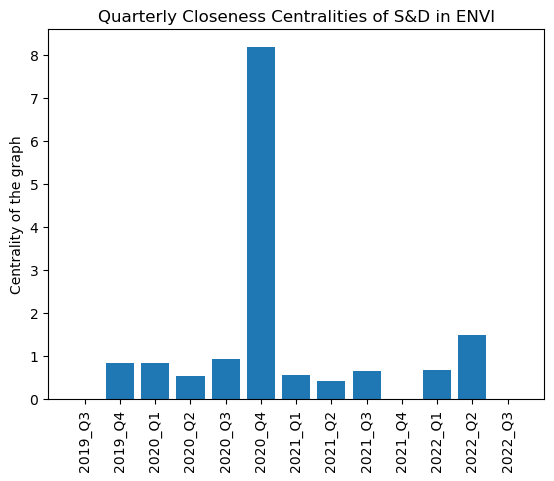
\includegraphics[width=\textwidth]{img/S&D_ENVI_Q_closeness.png}
	\end{column}
	
\end{columns}
\end{frame}

\begin{frame}{Our results: Centrality}
	
	Considering the \textbf{closeness} centralities of parties in the \textbf{quarterly} and \textbf{committee} division and only in the \textbf{biggest component}:
	\vspace{4mm}
	\pause
	
\begin{columns}
	\begin{column}{0.5\textwidth}
	Closeness of EPP party in ITRE greatest component:
	\\
	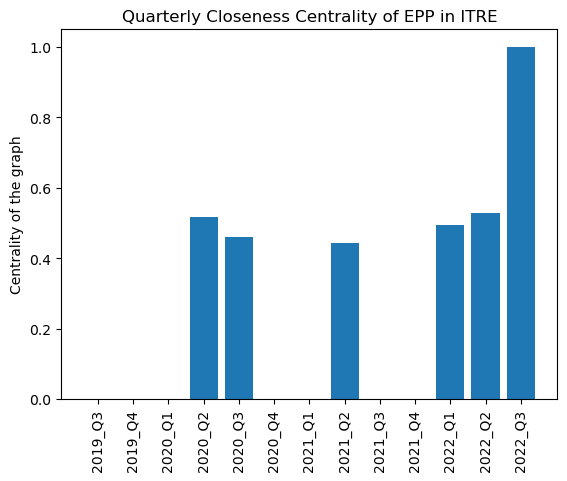
\includegraphics[width=\textwidth]{img/EPP_ITRE_Q_closeness_BIG.png}
	\end{column}
	
	\pause 
	\begin{column}{0.5\textwidth}
	Closeness of S\&D in ITRE greatest component:
	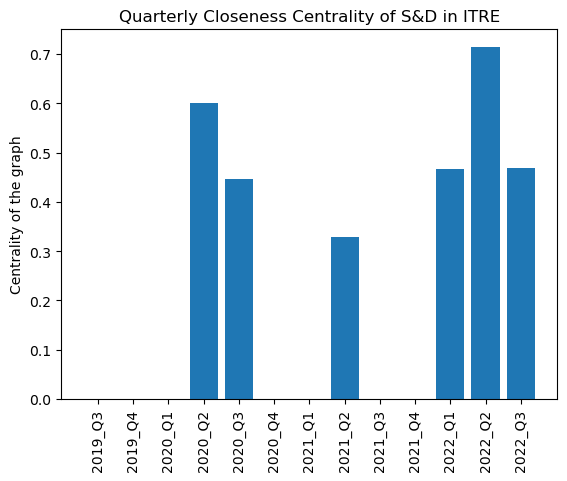
\includegraphics[width=\textwidth]{img/S&D_ITRE_Q_closeness_BIG.png}
	\end{column}
\end{columns}

\end{frame}

\begin{frame}{Our results: Centrality}
	
	Considering the \textbf{degree} centralities of parties in the \textbf{semesterly} division and only in the \textbf{biggest component}:
	\vspace{4mm}
	\pause
	
\begin{columns}
	\begin{column}{0.5\textwidth}
	Degree centrality of EPP in the largest component:
	\\
	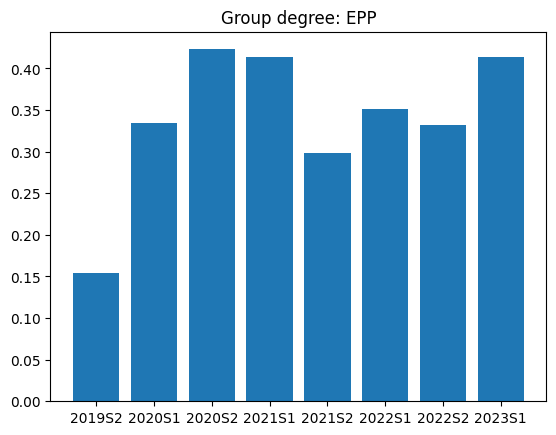
\includegraphics[width=\textwidth]{img/EPP_HY_deg.png}
	\end{column}
	
	\pause 
	\begin{column}{0.5\textwidth}
	Degree centrality of S\&D in the largest component:
	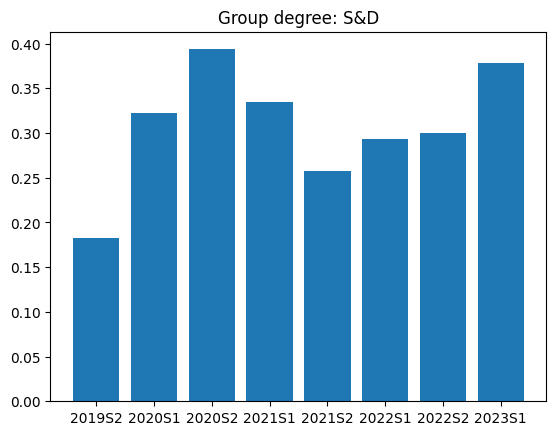
\includegraphics[width=\textwidth]{img/S&D_HY_deg.png}
	\end{column}
\end{columns}

\end{frame}

\begin{frame}{Our results: Centrality}
	
	It is especially interesting to consider the far-right Identity and Democracy Group (ID).
	 \textbf{degree} (left) and \textbf{closeness} (right) centralities the ID party in the \textbf{semesterly} division and only in the \textbf{biggest component}:
	\vspace{4mm}
	\pause
	
\begin{columns}
	\begin{column}{0.5\textwidth}
	Degree centrality of ID in the largest component:
	\\
	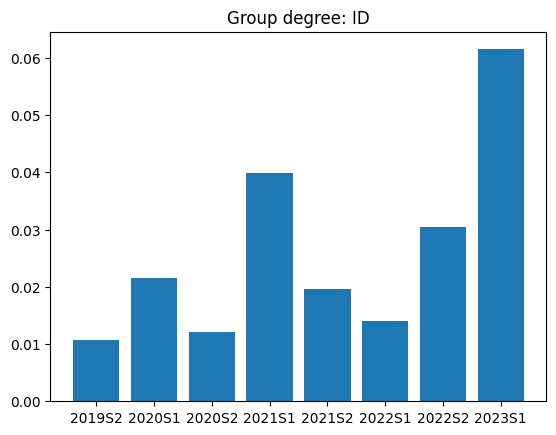
\includegraphics[width=\textwidth]{img/ID_HY_deg.png}
	\end{column}
	
	\pause 
	\begin{column}{0.5\textwidth}
	Closeness centrality of ID in the largest component:
	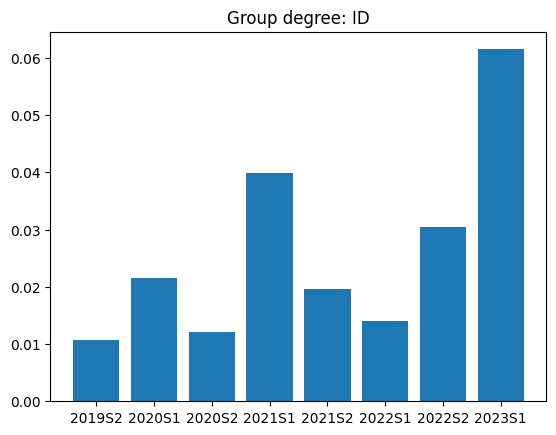
\includegraphics[width=\textwidth]{img/ID_HY_deg.png}
	\end{column}
\end{columns}

\end{frame}

\begin{frame}{Our results: Cohesion}
	We analyzed cohesion on a \textbf{semesterly basis}. \pause The data was too fractured for a more granular analysis.
	
	\vspace{1cm}
	
	\pause The semesterly analysis is a more useful way to aggregate the data because the work of the EP is naturally divided into semesters.
	
	\vspace{1cm}
	
	\pause General results: cohesion decreased across the board, with some exceptions.
\end{frame}

\begin{frame}{Our results: Cohesion}
	
	The cohesion of the \textbf{entire European Parliament}, across the given time period.
	
	\pause
	
	\vspace{0.5cm}
	
	\begin{columns}
		
		\begin{column}{0.5\textwidth}
			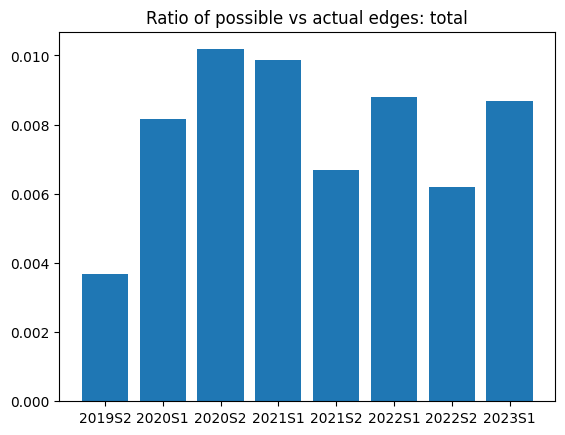
\includegraphics[width=\textwidth]{img/coh_all.png}
		\end{column}
	
	\end{columns}
\end{frame}

\begin{frame}{Our results: Cohesion}
	
	The cohesion of the two major parties, EPP and S\&D
	
	\pause
	
	\vspace{0.5cm}
	
	\begin{columns}
		
		\begin{column}{0.5\textwidth}
			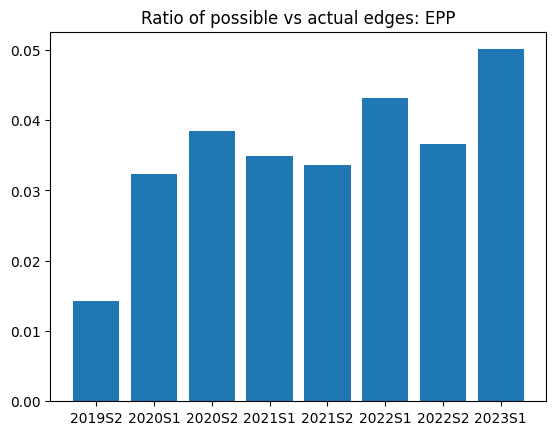
\includegraphics[width=\textwidth]{img/coh_epp.png}
		\end{column}
	
		\begin{column}{0.5\textwidth}
			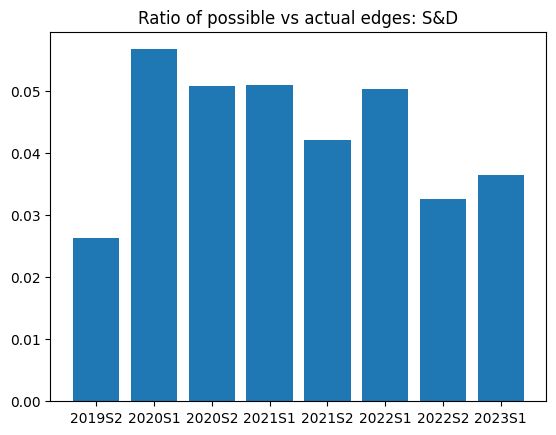
\includegraphics[width=\textwidth]{img/coh_s&d.png}
		\end{column}
		
	\end{columns}
\end{frame}

\begin{frame}{Our results: Cohesion}
	
	The cohesion of RE and GUE/NGL (both left-leaning parties)
	
	\pause
	
	\vspace{0.5cm}
	
	\begin{columns}
		
		\begin{column}{0.4\textwidth}
			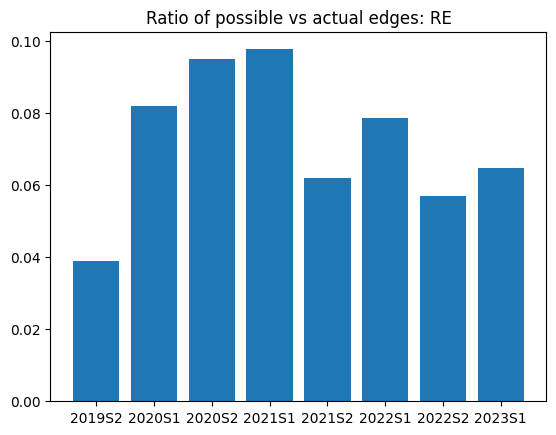
\includegraphics[width=\textwidth]{img/coh_re.png}
		\end{column}
		
		\begin{column}{0.4\textwidth}
			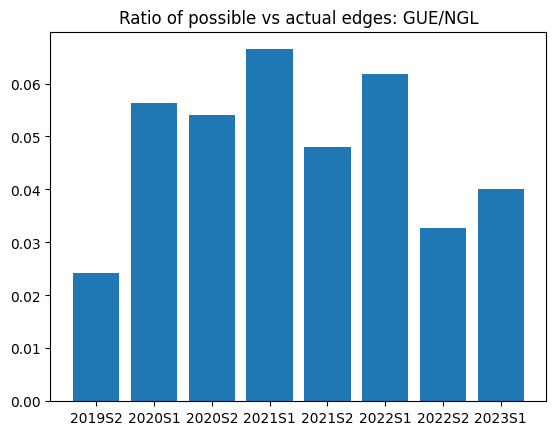
\includegraphics[width=\textwidth]{img/coh_guengl.png}
		\end{column}
			
	\end{columns}
	
	\vspace{0.5cm}
	
	\pause We see a notable decrease over time
\end{frame}

\begin{frame}{Our results: Cohesion}
	
	The cohesion of ECR and ID (both right-wing parties)
	
	\pause
	
	\vspace{0.5cm}
	
	\begin{columns}
		
		\begin{column}{0.4\textwidth}
			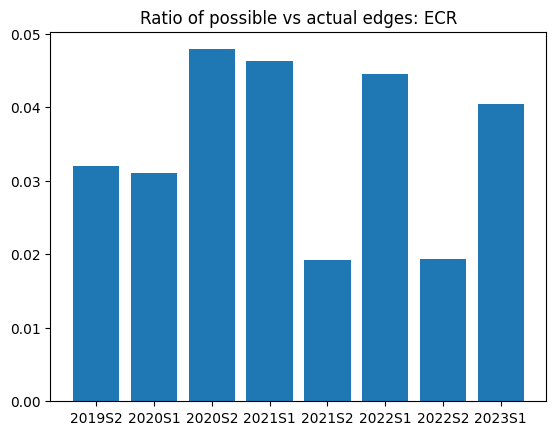
\includegraphics[width=\textwidth]{img/coh_ecr.png}
		\end{column}
		
		\begin{column}{0.4\textwidth}
			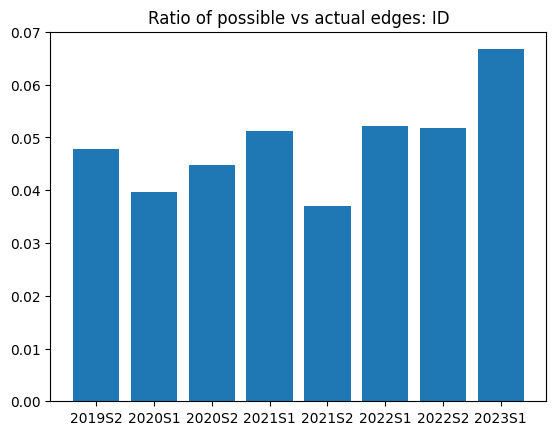
\includegraphics[width=\textwidth]{img/coh_id.png}
		\end{column}
		
	\end{columns}
	
	\vspace{0.5cm}
	
	\pause We mostly see stagnation
\end{frame}

\begin{frame}{Our results: Cohesion}
	
	The cohesion of the Greens (left-leaning `green' party)
	
	\pause
	
	\vspace{0.5cm}
	
	\begin{columns}
		
		\begin{column}{0.4\textwidth}
			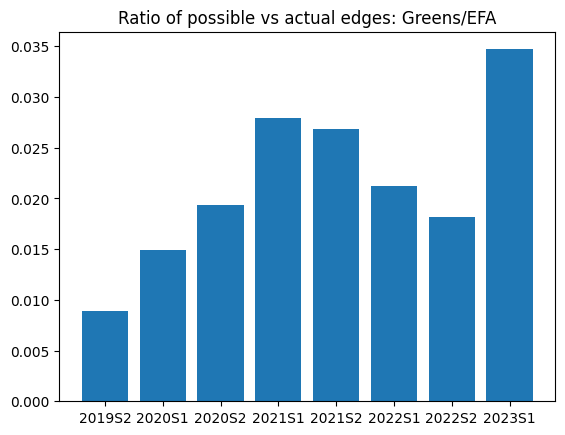
\includegraphics[width=\textwidth]{img/coh_greens.png}
		\end{column}
		
		
	\end{columns}
	
	\vspace{0.5cm}
	
	\pause This one shows no clear trends\pause, and the spike in the last semester is mysterious and unexplained
\end{frame}

\begin{frame}{Cohesion conclusions}
	
	\pause The `rise of the right-wing' phenomenon is observed\pause, left-wing parties are losing cohesion
	
	\vspace{0.5cm}
	
	\pause Some parties show alternation between first and second semesters of each year, some parties don't
	
	\vspace{0.5cm}
	
	\pause The overall cohesion of the network is decreasing
	
\end{frame}

\begin{frame}{Final conclusions}
	
	\pause Right-wing parties are gaining prominence across the board
	
	\vspace{0.5cm}
	
	\pause The liberal RE party lost its previous ``bridge" status\pause, instead it seems that EPP is now the bridge between the left and right wings
	
	\vspace{0.5cm}
	
	\pause The future of the EP is probably going to be decided by a right-wing coalition
	
\end{frame}

\begin{frame}{}
	
	\centering Thanks for watching
	
\end{frame}


\end{document}
